\documentclass[12pt]{article}

\usepackage{lineno}


\usepackage[hmargin=1.5cm,vmargin=1.5cm]{geometry}

\usepackage[affil-it]{authblk}
\usepackage[percent]{overpic}
\usepackage{float}
\usepackage{color}
\usepackage{hyperref}
\usepackage[numbers,sort&compress]{natbib}

\title{Beam test of the silicon timing for use in calorimetry.}

\author[1]{A.~Apresyan}
\author[2]{G.~Bolla}
\author[3]{H.~Kim}
\author[2]{S.~Los}
\author[1]{C.~Pena}
\author[1]{F.~Presutti}
\author[2]{E.~Ramberg}
\author[2]{A.~Ronzhin}
\author[1]{M.~Spiropulu}
\author[1]{S.~Xie}
\affil[1]{California Institute of Technology, Pasadena, CA, USA}
\affil[2]{Fermi National Accelerator Laboratory, Batavia, IL, USA}
\affil[3]{University of Chicago, Chicago, IL,  USA}

\date{}

\begin{document}
\linenumbers
\maketitle

\abstract{The high luminosity upgrade of the Large Hadron Collider (HL-LHC) at
CERN is expected to provide instantaneous luminosities of $5\times 10^{34}$
cm$^{-2}$ s$^{-1}$. Collision at the high luminosity has shorter bunch spacing
and more pileup [PU] events in the complex luminous regions. Precision timing
allows extend calorimetric measurements into high density environment. We
performed some study of the possible options to improve timing for
calorimetry~\cite{Anderson:2015gha, MCPFastCaloNIMA, Ronzhin2015288,
Ronzhin201552}. CMS calorimetry upgrade based on silicon as sensitive layer is
another upgrade option~\cite{Butler:2020886}. Signal response of silicon
detectors could be about few ns with rise time of $\sim$1 ns. 8000 e-h pairs
produced in silicon per 100 $\mu$m, which is much higher than silicon noise  .
These properties with relatively high radiation hardness~\cite{CMSPreshower} allow to use
silicon in calorimetric detectors. In this article we present results of
timing study of silicon produced by Hamamatsu~\cite{hamamatsu}.}


\section{Introduction} 

One way to mitigate the pileup confusion effects, complementary to precision
tracking methods, is to perform a time of arrival measurement associated with a
particular layer of the calorimeter, allowing for a time assignment for both
charged particles and photons. Such a measurement with a precision of about
20-30 ps, when unambiguously associated to the corresponding energy measurement,
will significantly reduce the inclusion of pileup particles in the
reconstruction of the event of interest, given that the spread in collision time
of the pileup interactions is approximately 200~ps. The association of the time
measurement with the energy measurement is crucial, and leads to a prototype
design that calls for the time and energy measurements to be performed in the
same active detector element. It is in this context that we studied the
possibility of measuring the time of arrival of the particles with a
calorimetric device when using silicon as sensitive element. The paper is organized as follows. The general silicon timing properties are
described and bench test results of the used silicon described in
Section~\ref{sec:siliconpad}. Test beam setup are presented in
Section~\ref{sec:tbeam}, and the results of the silicon test are presented in
Section~\ref{sec:results}. Sections~\ref{sec:discussion} and
~\ref{sec:conclusion} are devoted to discussion and conclusion, respectively.
\section{Silicon timing. Bench test of used silicon}
\label{sec:siliconpad}

Few factors determine the timing response of silicon detectors. One of them
defines time constant and depends on series resistance of the silicon, load
resistance and terminal capacitance. The other are due to silicon intrinsic
properties: the silicon thickness, the carrier’s velocity and its collection
time, dependent on depletion voltage and type of the carriers. The carriers
drift time in fully depleted silicon determines the carrier’s collection time.
This time determines the silicon time response in case of small time constant,
but the response could be mostly dependent on time constant for silicon with
large capacitance.We used for our test the silicon, produced by Hamamatsu~\cite{hamamatsu}. The
thickness of the silicon is ~325 $\mu$m. The transverse size of the silicon is
6x6 mm$^2$. The negative bias voltage was applied to p-side of the silicon. The
dependence of the diode capacitance on the bias voltage is presented in
Fig.~\ref{fig:SiliconDiode}. The junction capacitance depends on the area of
p-layer and the thickness of the depletion layer which increased with inverse
bias voltage. When charged particle pass through the silicon the produced
electrons collected on the opposite (to p-side) n-side of the silicon and forms
the output signal. The electrical schematics of the silicon diode and
capacitance dependence on bias voltage presented in Fig.~\ref{fig:SiliconDiode}.


\begin{figure}[htbp] 
\centering
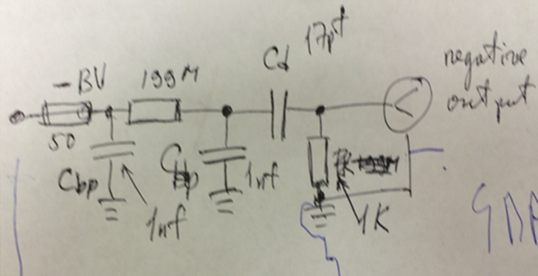
\includegraphics[width=0.45\textwidth]{plots/SiliconDiodeDiagram.png} 
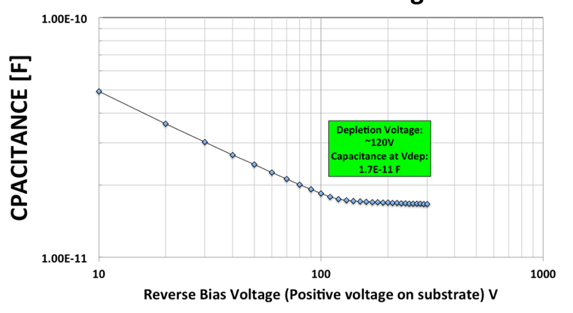
\includegraphics[width=0.45\textwidth]{plots/SiliconDiodeCV.png} 
\caption{Electrical schematics of the silicon diode (left) and it capacitance in dependence on bias voltage (right). } 
\label{fig:SiliconDiode} 
\end{figure} 
The silicon box and bench test setup presented in Fig.~\ref{fig:SiliconPad}. Measurements were performed at SiDet facility of Fermilab. The sensitivity of the silicon diode to light was tested to check it functionality.\begin{figure}[htbp] 
\centering
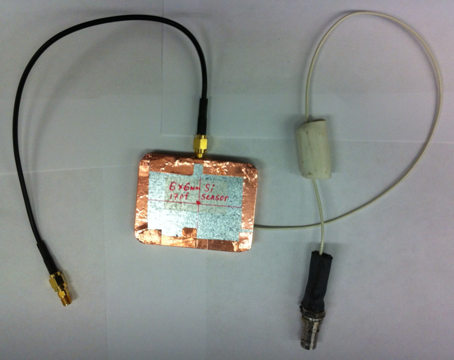
\includegraphics[width=0.45\textwidth]{plots/SiliconPadExternalView.png} 
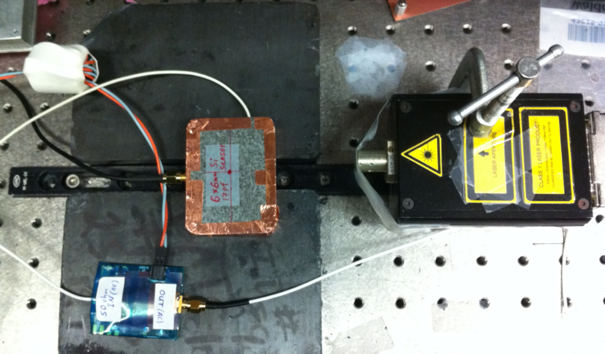
\includegraphics[width=0.45\textwidth]{plots/SiliconPadBench.png} 
\caption{External view of the box with silicon diode and PC board inside (left) and bench test setup (right).} 
\label{fig:SiliconPad} 
\end{figure} 

The silicon diode was placed in the metal box. The HV was applied to the PC
board by the cable terminated by HSV connector. The silicon diode output signal
was taken out by using the SMA connector attached to the box. Dark current
dependence on bias voltage was tested. The maximum value of the current at -500
V of the bias was less of 1nA. (we had not in hands picoampermeter to measure
the current). \section{Test beam setup and results of the silicon test }
\label{sec:tbeam}

The test beam measurements were performed in FTBF. The main parts of the setup are well described in Refs.~\cite{Anderson:2015gha, MCPFastCaloNIMA, Ronzhin2015288,
Ronzhin201552}. For the measurement with silicon it was slightly modified as shown in Fig.~\ref{fig:SiliconPadTBeam}.

\begin{figure}[htbp] 
\centering
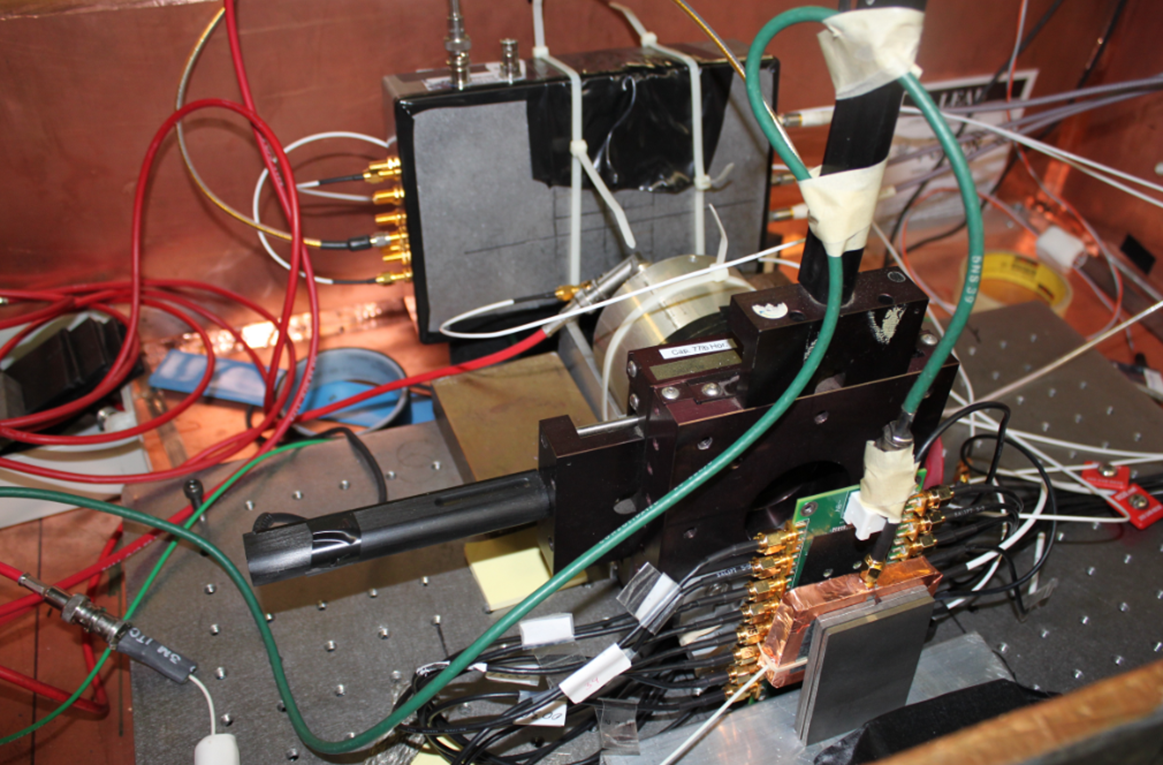
\includegraphics[width=0.8\textwidth]{plots/SiliconPadTestBeam.png} 
\caption{Test beam setup.} 
\label{fig:SiliconPadTBeam} 
\end{figure} 

The test beam setup is shown in Fig.~\ref{fig:SiliconPadTBeam}. The silicon
detector was placed inside of the metal box. The absorber (W or Pb) was placed
upstream for measurements with electron beam. We have not used absorber in
measurements with 120 GeV protons. Other detectors which shown in the
Fig.~\ref{fig:SiliconPadTBeam} were tested simultaneously. The setup contains a data acquisition (DAQ) system based on CAEN V1742 5 Gs/s
digitizer~\cite{CAENDRS}, HV power supplies, and equipment to monitor and
control test beam parameters. The dark box was located on a moving table
allowing us to change the box position both in the horizontal and vertical
direction in the range of 300 mm in X and Y with an accuracy better than 0.5 mm.
Event selection and analysis was described in detail in
Ref.~\cite{MCPFastCaloNIMA}. The trigger was based on a scintillation counter
with 1.8 x 2 mm2 transverse size. \textbf{DO WE NEED TO TALK ABOUT THESE The
three detectors (4x4 Hamamatsu MPPC matrix [16], Photek 240 timing reference
MCP-PMT and 6x6 cm2 LAPD [17])} were placed in line downstream of the tested
silicon. The silicon detector was positioned on an X-Y moving stage, which
allowed movement in both X and Y directions by $\pm$15mm. The stage was operated
remotely from the test beam control room. It was possible to align the silicon
detector with ~10 $\mu$m accuracy in both X and Y directions. The tungsten absorber material was used to initiate an electromagnetic shower
when high energy electrons pass through. Signals from the detectors and the
Cherenkov counter used for electron identification were split by high frequency
Mini-Circuits ZFRSC-42-S þ splitters (4.2 GHz BW). The outputs were connected to
CAEN V1742 digitizer, which allowed to hook up 32 channels for the measurements.
The schematic of the similar readout (with DRS4) is described in detail in~\cite{Anderson:2015gha}. 

\section{Test Beam Measurements and Results} 
\label{sec:results} 

Measurements were performed using the secondary beam at the FTBF, which provides
a beam of electrons and pions. Beam energies ranging from 4 GeV/c$^2$ to 32 GeV/c$^2$
were used, for which the electron purity ranges between 70\% at the lowest
energy to about 10\% at the highest energy. Stacks of tungsten plates with
different thicknesses were placed immediately upstream of the silicon device in
order to measure the response along the longitudinal direction of the
electromagnetic shower. The transverse size of the tungsten plates allowed us to
fully cover the transverse size of the silicon device. The signals from the
silicon sensor and the Photek MCP-PMT are read out and digitized by the V1742
digitizer, and example signal waveforms are shown in Fig.~\ref{fig:pulses}.

\begin{figure}[htbp] 
\centering
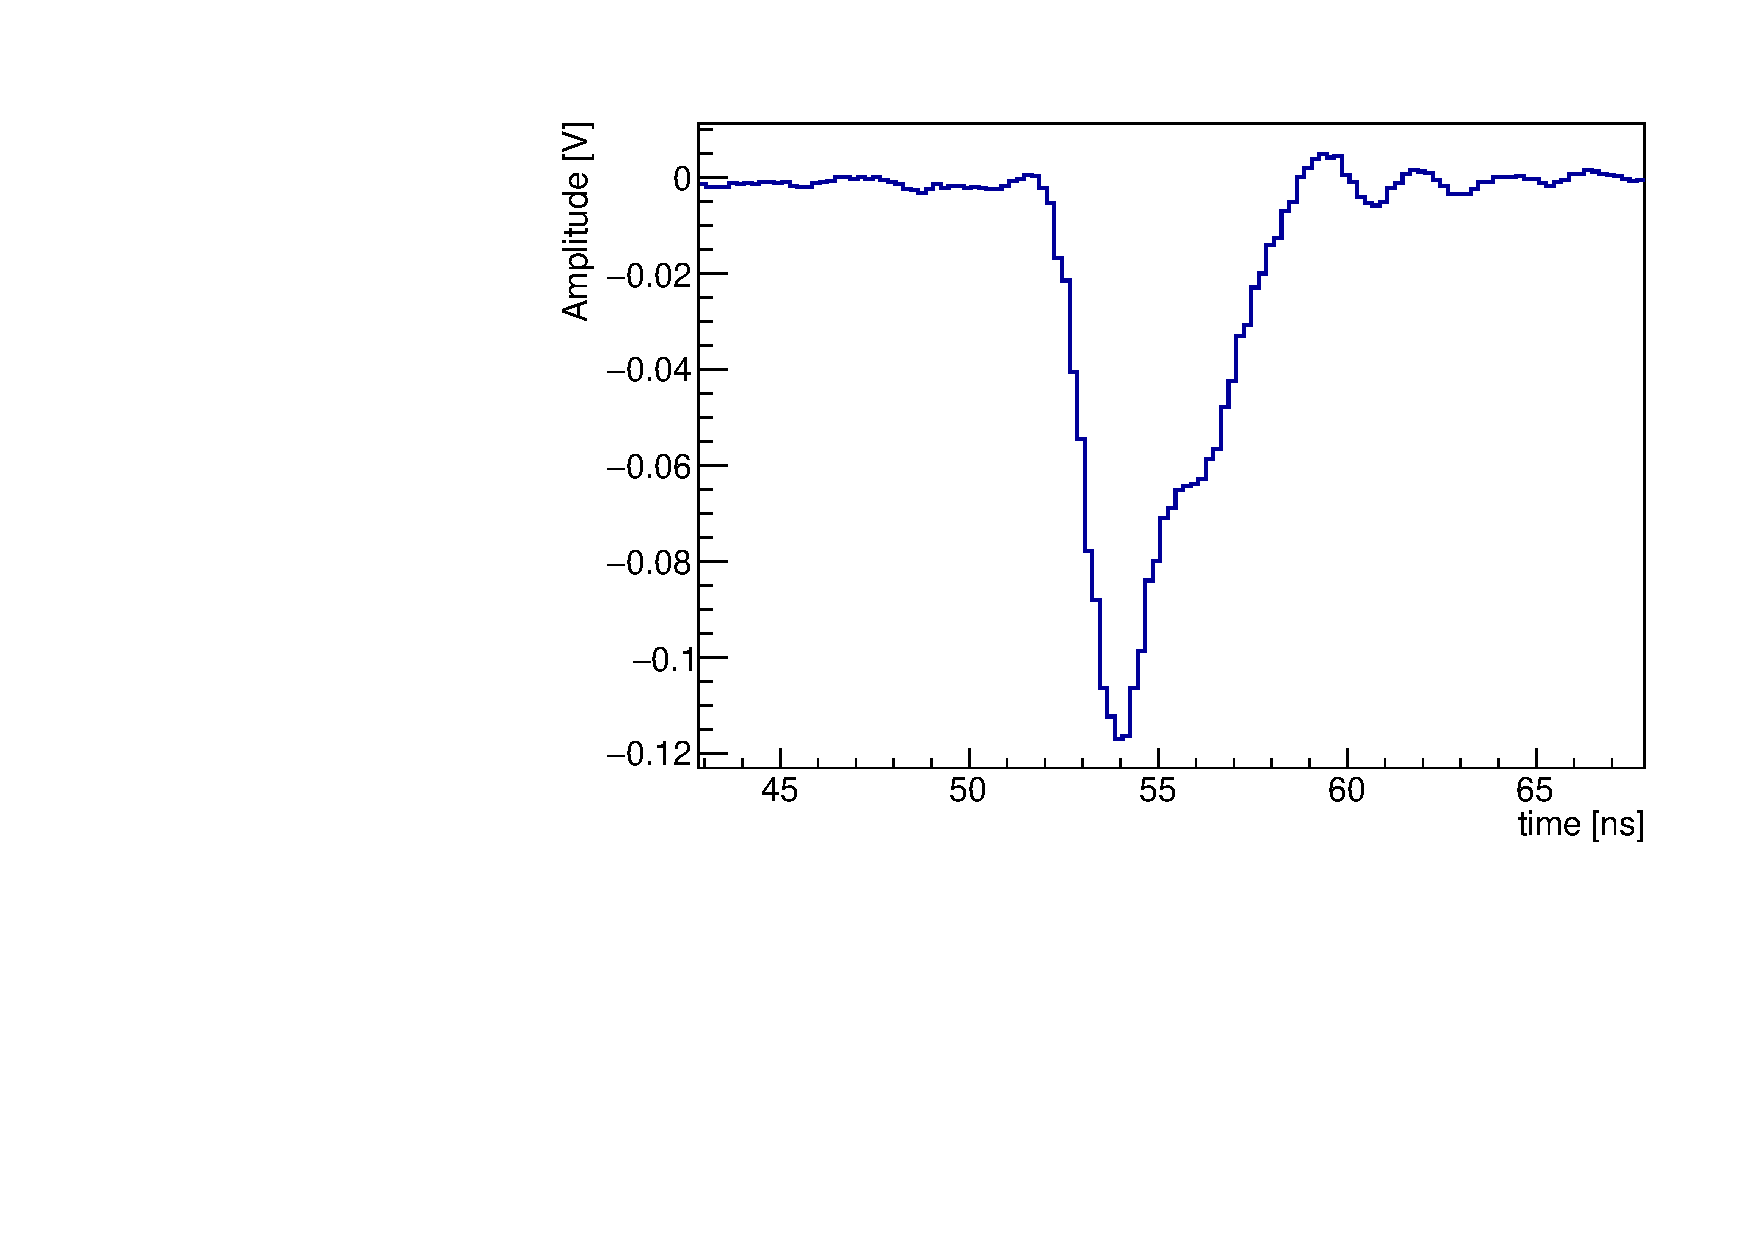
\includegraphics[width=0.45\textwidth]{plots/ExampleSiliconPadPulse_6X0_16GeV.pdf} 
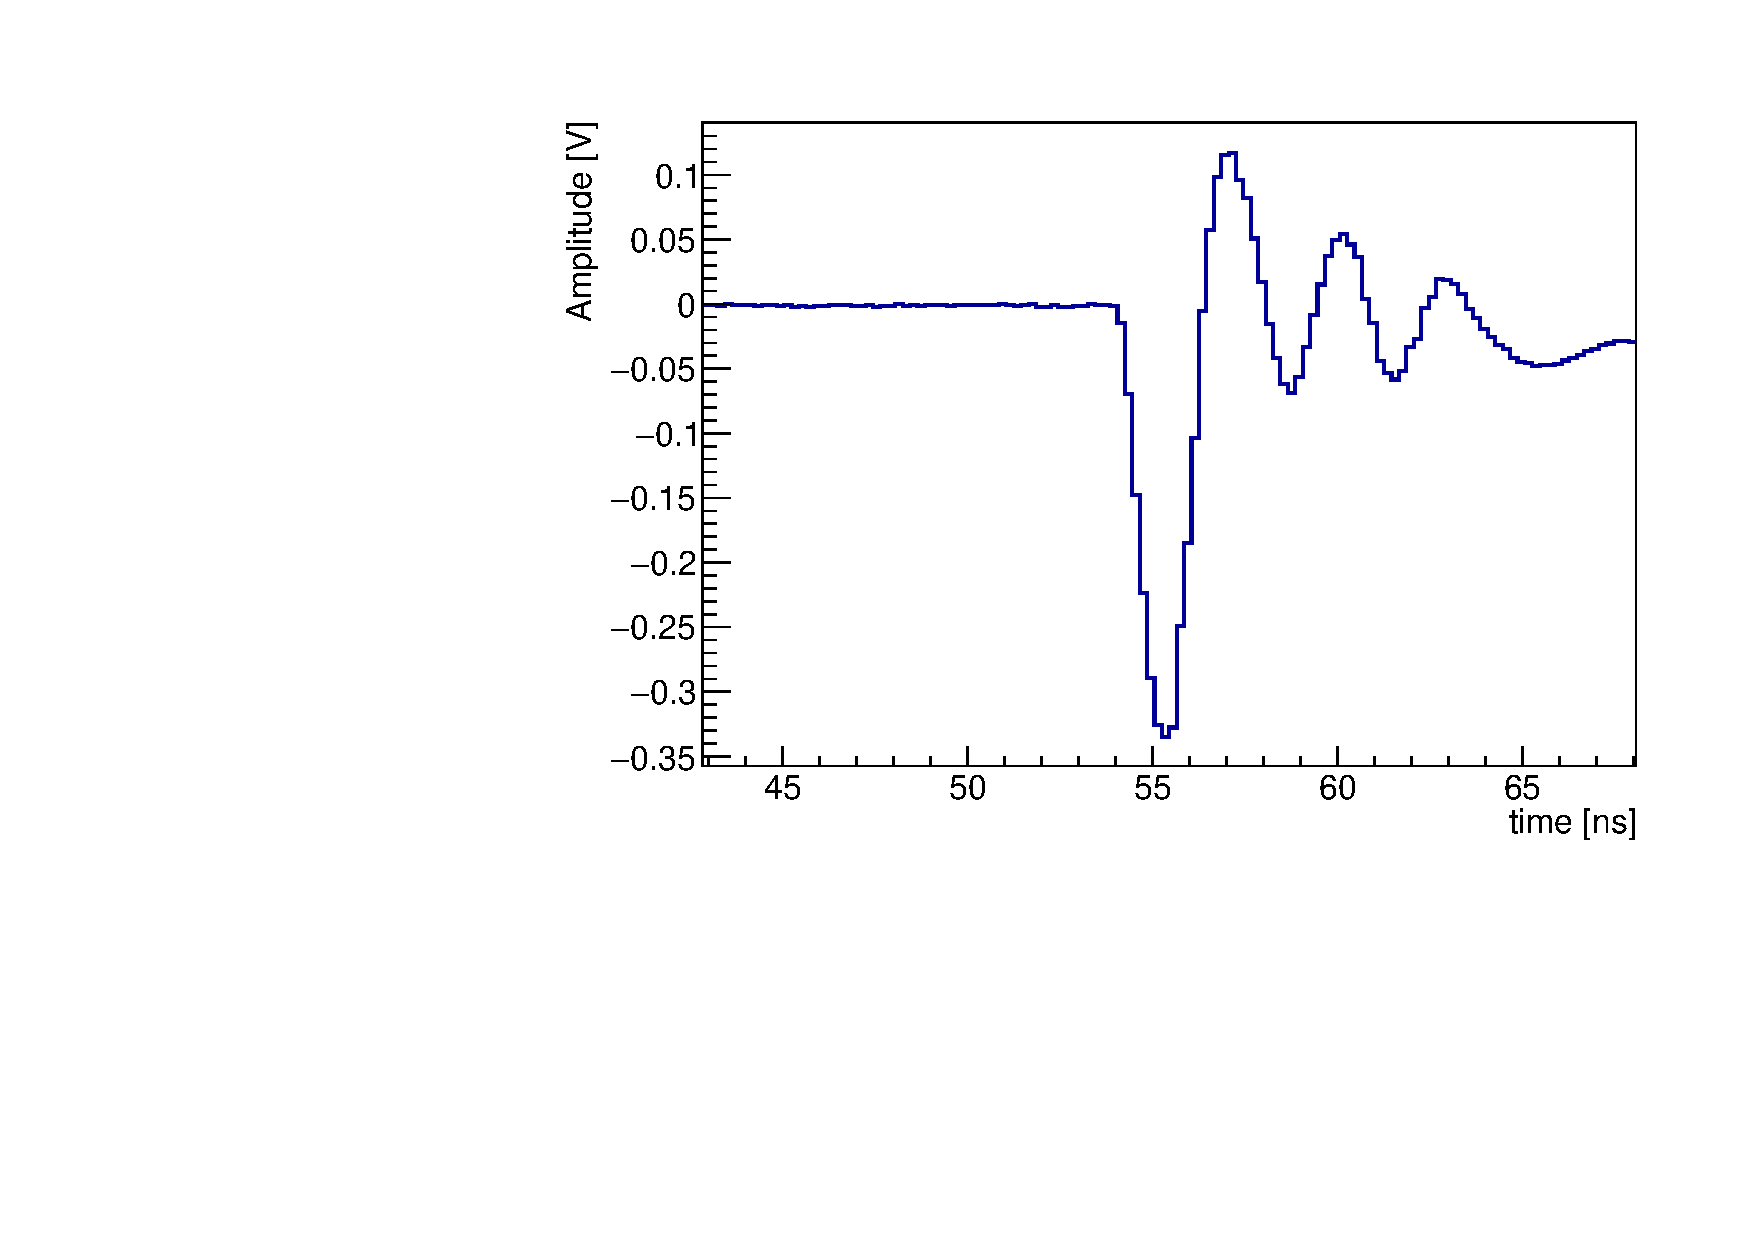
\includegraphics[width=0.45\textwidth]{plots/ExamplePhotekPulse.pdf} 
\caption{Examples of the signal pulse waveform for the silicon sensor (left) and the Photek MCP-PMT (right) digitized by CAEN V1742 digitizer board.} 
\label{fig:pulses} 
\end{figure} 

The raw waveforms are calibrated in both the voltage and time dimension using
known inputs from a pulse generator~\cite{Kim201467}. The total collected charge for each
signal pulse is computed by integrating a 10-ns window around the peak of the
pulse. The time for the reference Photek MCP-PMT detector is obtained by fitting
the peak region of the pulse to a Gaussian function and the mean parameter of
the Gaussian is assigned as the timestamp. The time for signals from the silicon
sensor is obtained by performed a linear fit to the rising edge of the pulse and
the time at which the pulse reaches 30\% of the maximum amplitude is assigned as
its timestamp. We measured the “electronic” time resolution (TR) of the CAEN
V1742 digitizer as $\sim$4~ps and neglected this impact on the timing measurements
described below.

Electrons were identified using a combination of the gas Cherenkov counter
provided by the FTBF and the signal size in the Photek detector located further
downstream of the silicon sensor. Electromagnetic showers induced by electrons
produce significantly larger signals in the Photek MCP-PMT, while pions produce
a much smaller signal. After imposing the electron identification 
requirements the electron purity is between $80\%$ and $90\%$ for all beam
conditions. 

%% The gain of the silicon detector with the amplifiers was
%% in excess of $10^{6}$. Placement of absorbers in front of the silicon also increased
%% the signal size due to increased particle flux from secondary shower particles. We can estimate the 
%% amplitude of the silicon signal for 120 GeV proton. The
%% amount of electron produced is ~30000 in 300 um silicon. The gain of used
%% amplifiers (2 Ortec 120V in series) is 200. The total gain of the circuit is
%% $6\times 10^6$ electrons. The corresponding charge is 1 pC/proton. Taking into account
%% the pulse duration (which is $\sim$5ns), external load 50 Ohm and factor of 2 for
%% triangular signal shape we obtain 20 mV/proton the silicon signal amplitude.
%% This estimation consistent with the measurement.

We begin by establishing the signal characteristics of a minimum-ionizing
particle (MIP) using beams of 120 GeV protons as well as 8 GeV electrons with no
absorbers upstream of the silicon pad sensor. To distinguish MIP signals from
noise, we collect data events of pure noise with no beam and random triggers.
The charge distribution for noise runs is presented in
Fig.~\ref{fig:noise}. As expected, the charge distribution for noise
runs is centered at 0, and the RMS is about $2$~fC. 

\begin{figure}[htbp] 
\centering
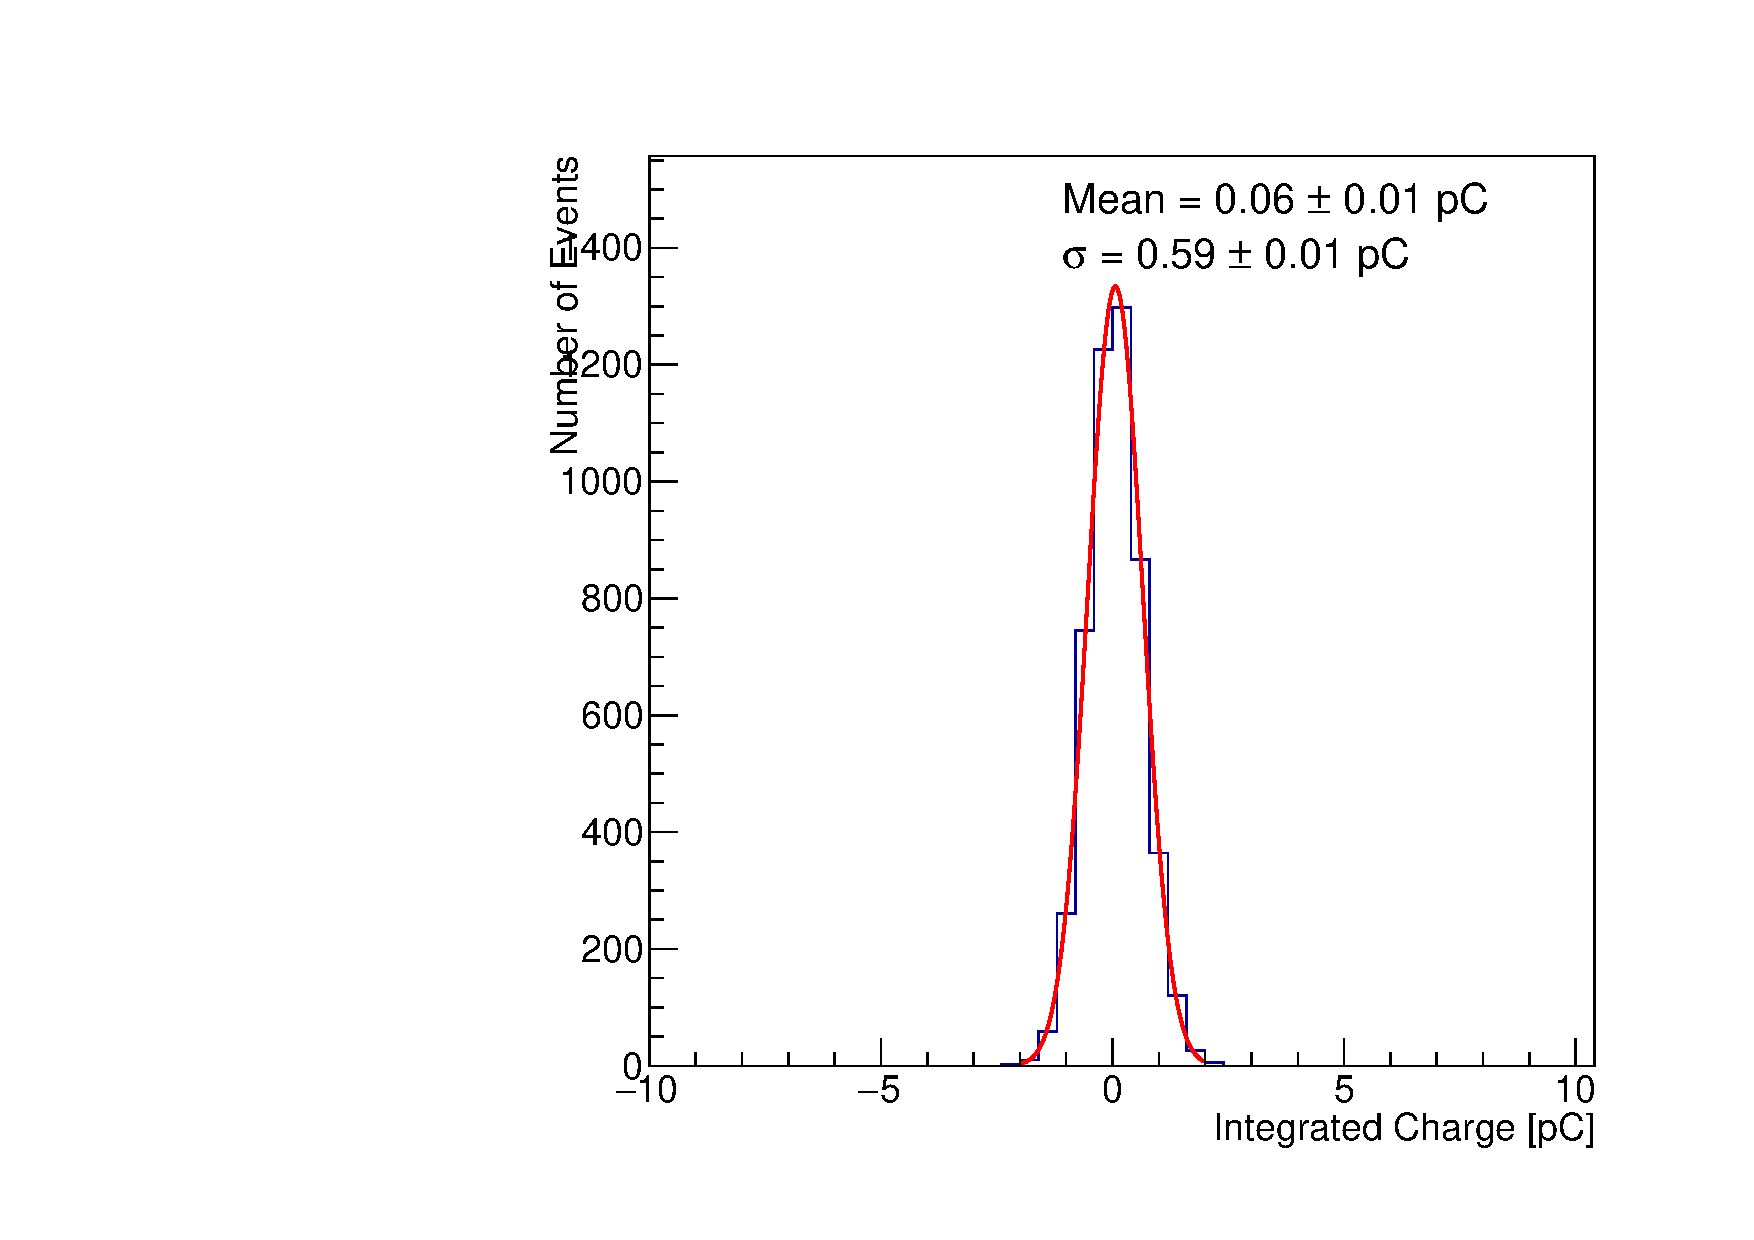
\includegraphics[width=0.45\textwidth]{plots/NoiseNoBeam_charge.pdf} 
\caption{The distribution of charge integrated in the silicon sensor is shown for randomly triggered 
data recorded with no beam. } 
\label{fig:noise} 
\end{figure} 

In Figure~\ref{fig:MIP}, we show the response of the silicon sensor to
the proton and electron beam without any absorbers upstream. We observe very similar
response for these two cases, and measure an integrated charge of $4.5$~fC and $5.0$~fC
for the proton and electron beams respectively. The measured charge takes into account
the response of the amplifiers and attenuators used, which were measured 
in the lab using a pulse generator in the full dynamic range relevant for the current study.
We expect that a MIP traversing a silicon sensor of thickness 300$\mu$m to produce roughly 32000 
electron-hole pairs, corresponding to a charge of about $5.1$~fC. Thus, our measured value
is in close agreement with expectations. Having established the absolute scale of the measured 
response using MIP's, in our remaining studies we normalize all charge measurements to the 
charge integrated in the silicon sensor for one MIP. 

\begin{figure}[htbp] 
\centering
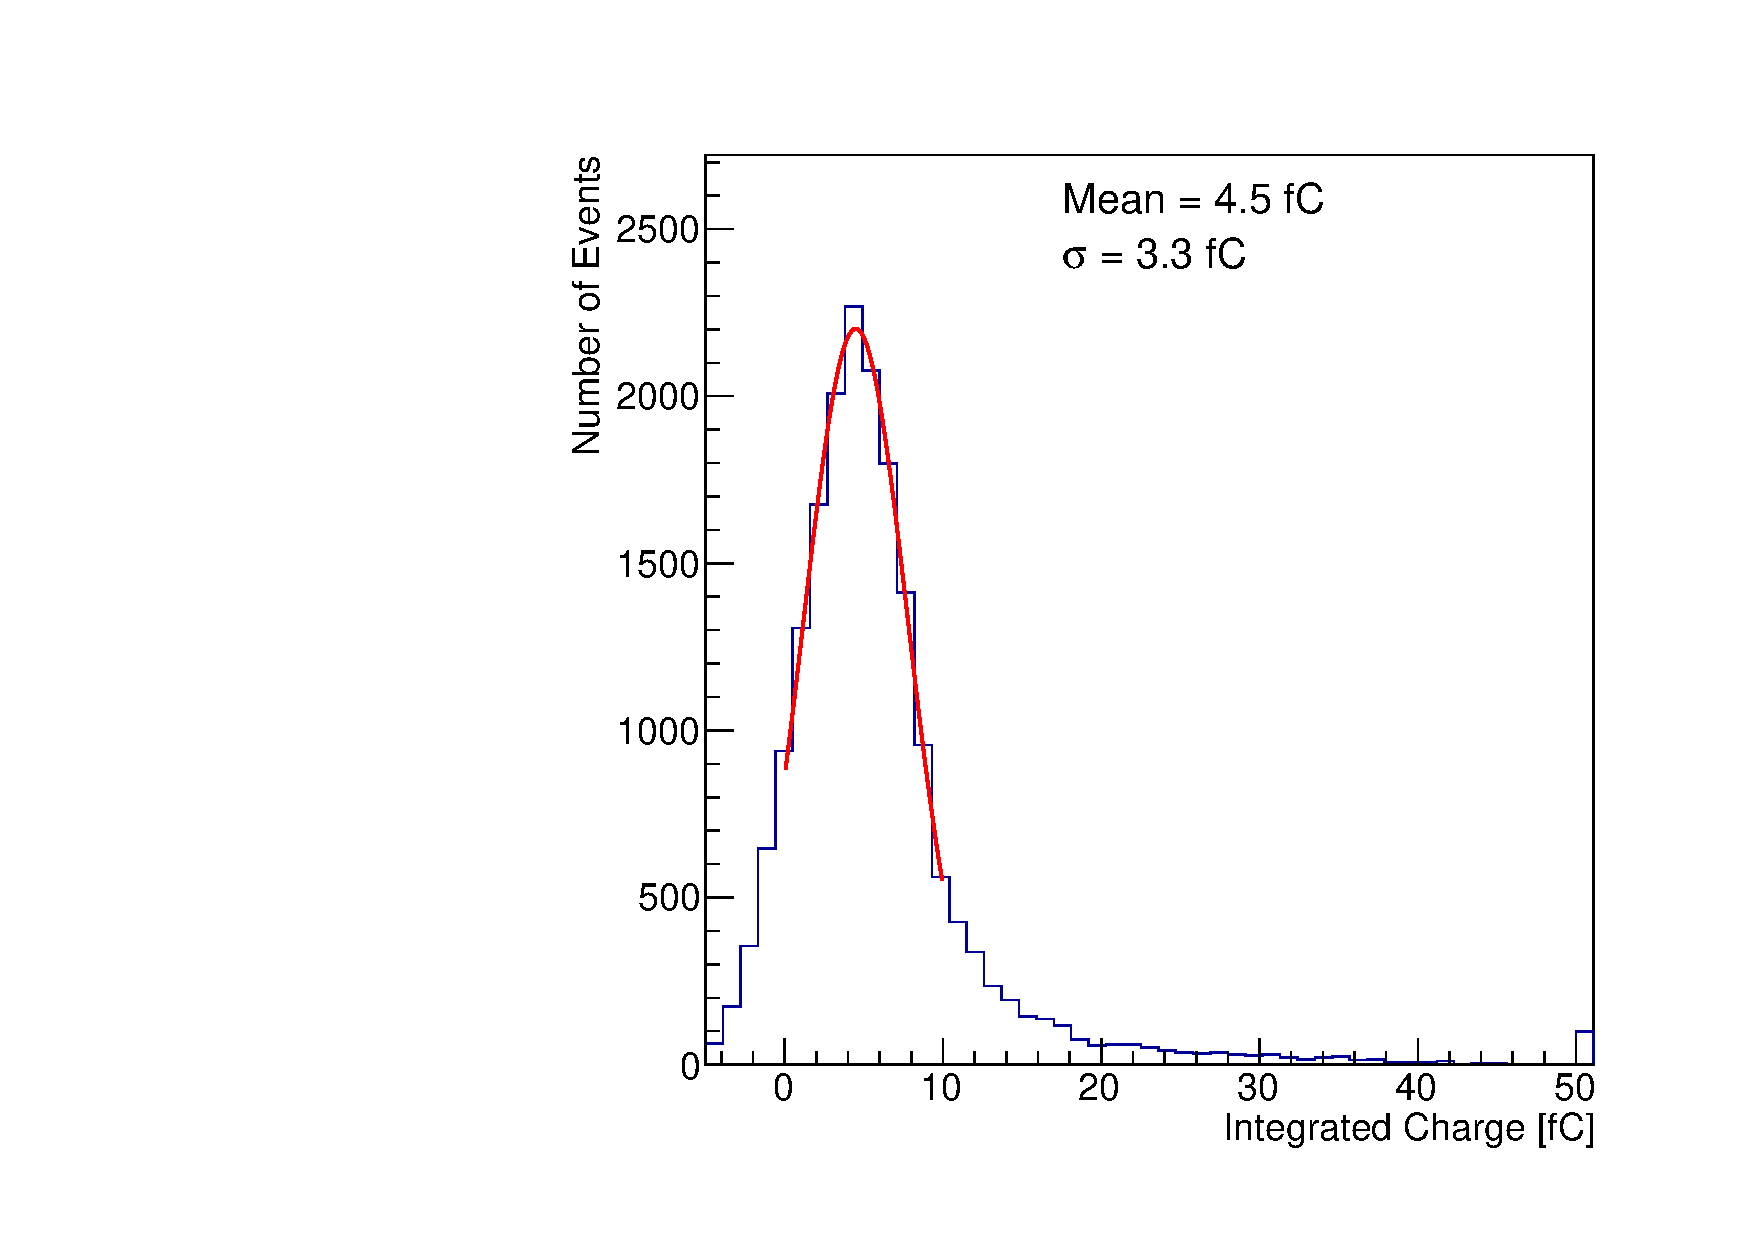
\includegraphics[width=0.45\textwidth]{plots/Proton_charge.pdf} 
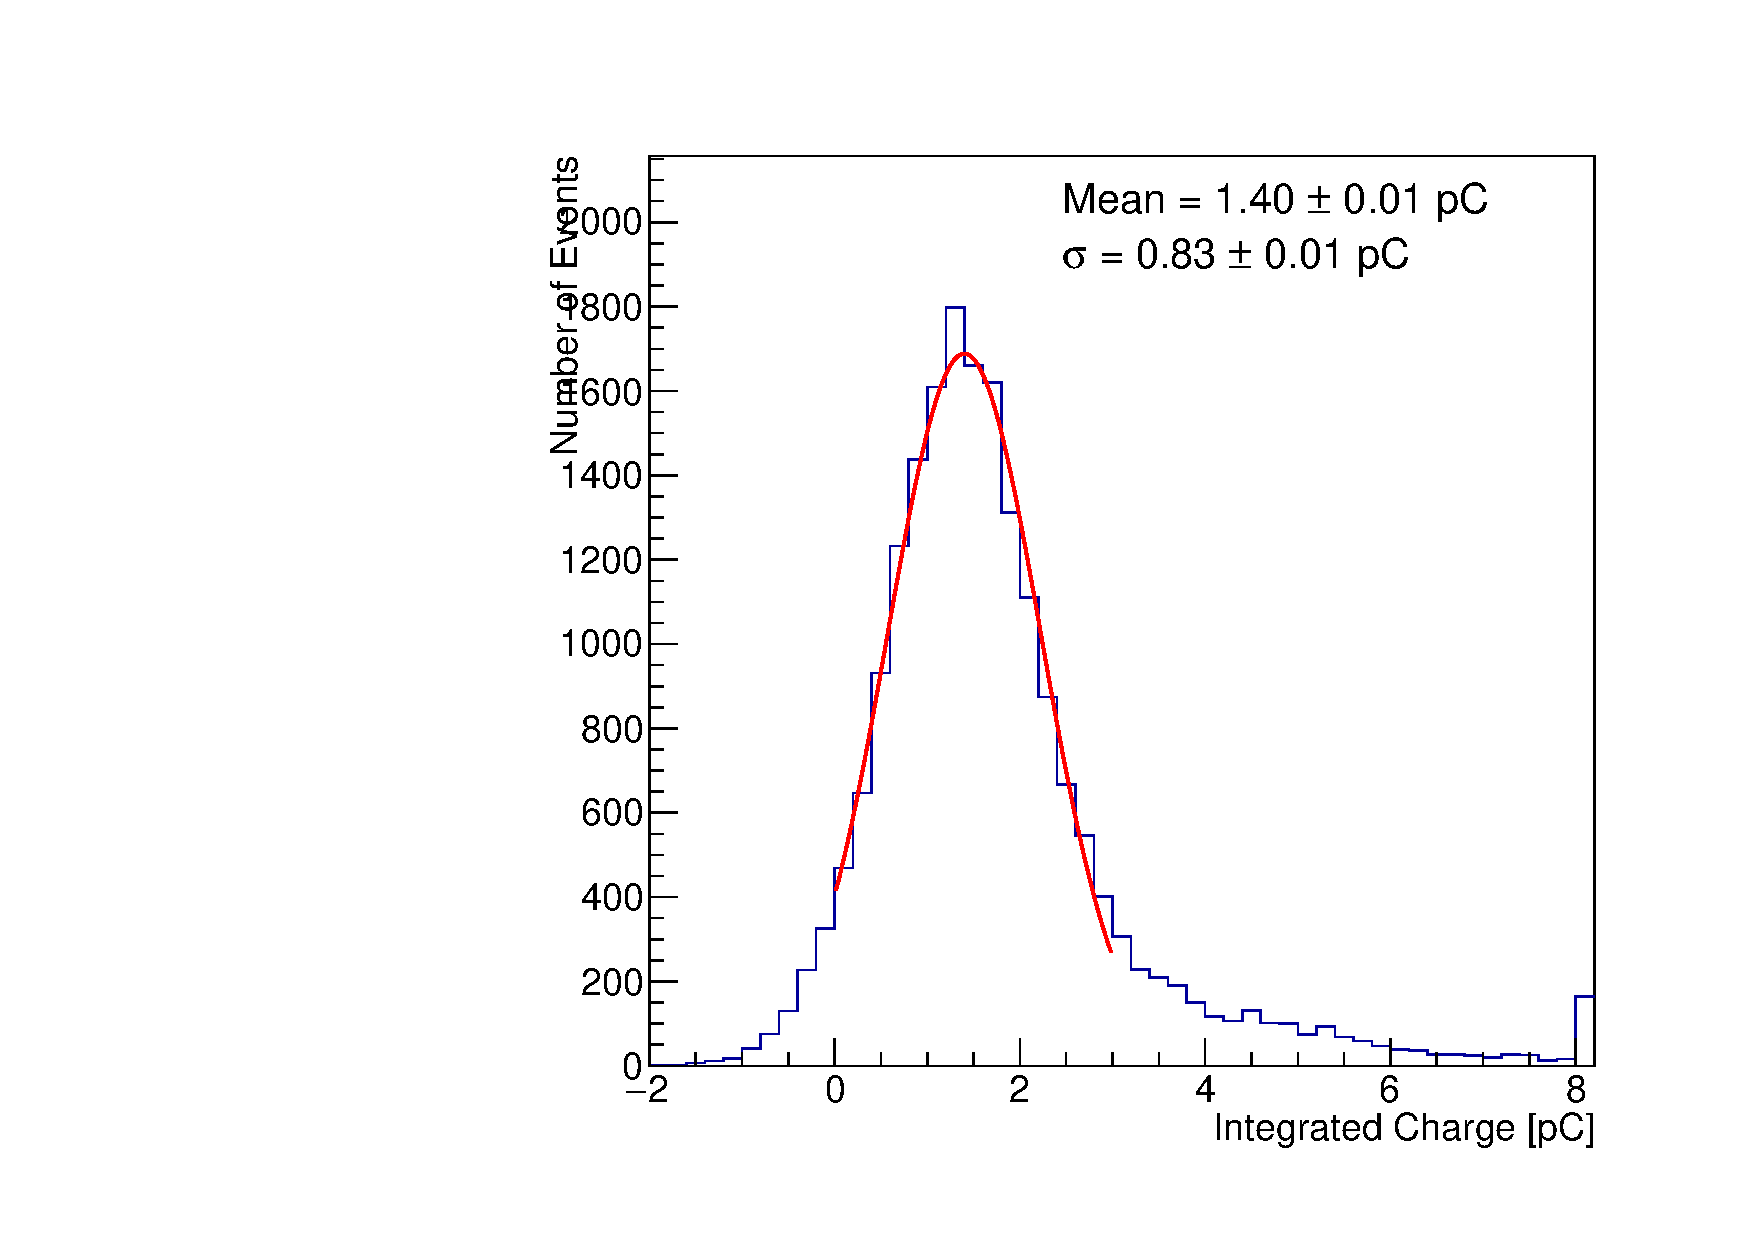
\includegraphics[width=0.45\textwidth]{plots/Electron_0X0_charge.pdf} 
\caption{The distribution of charge integrated in the silicon sensor is shown
for a beam of $120$~GeV protons (left) and $8$~GeV electrons (right) without
any absorber upstream of the silicon sensor. These conditions mimic the response
of the silicon sensor to a minimum-ionizing particle. 
} 
\label{fig:MIP} 
\end{figure} 

We study the response of the silicon sensor to electron beams of various energies after
6 radiation lengths of tungsten absorber. The silicon sensor is expected to be
sensitive to the number of secondary electrons produced within the electromagnetic
shower, and therefore its response is expected to scale up with higher incident
electron energy. In Figure~\ref{fig:ChargeDistributionExample}, we show
an example of the integrated charge distribution measured in the silicon sensor
after 6 radiation lengths of tungsten for $32$~GeV electrons. We plot the mean 
and RMS of these distributions as a function of incident electron beam energy
in Figure~\ref{fig:MIPVsEnergy}. The uncertainties plotted show the RMS
of the charge distribution. We observe a fairly linear depedence between
the measured charge and the incident beam energy, for beam energies
between $4$~GeV and $32$~GeV. 

\begin{figure}[htbp] 
\centering
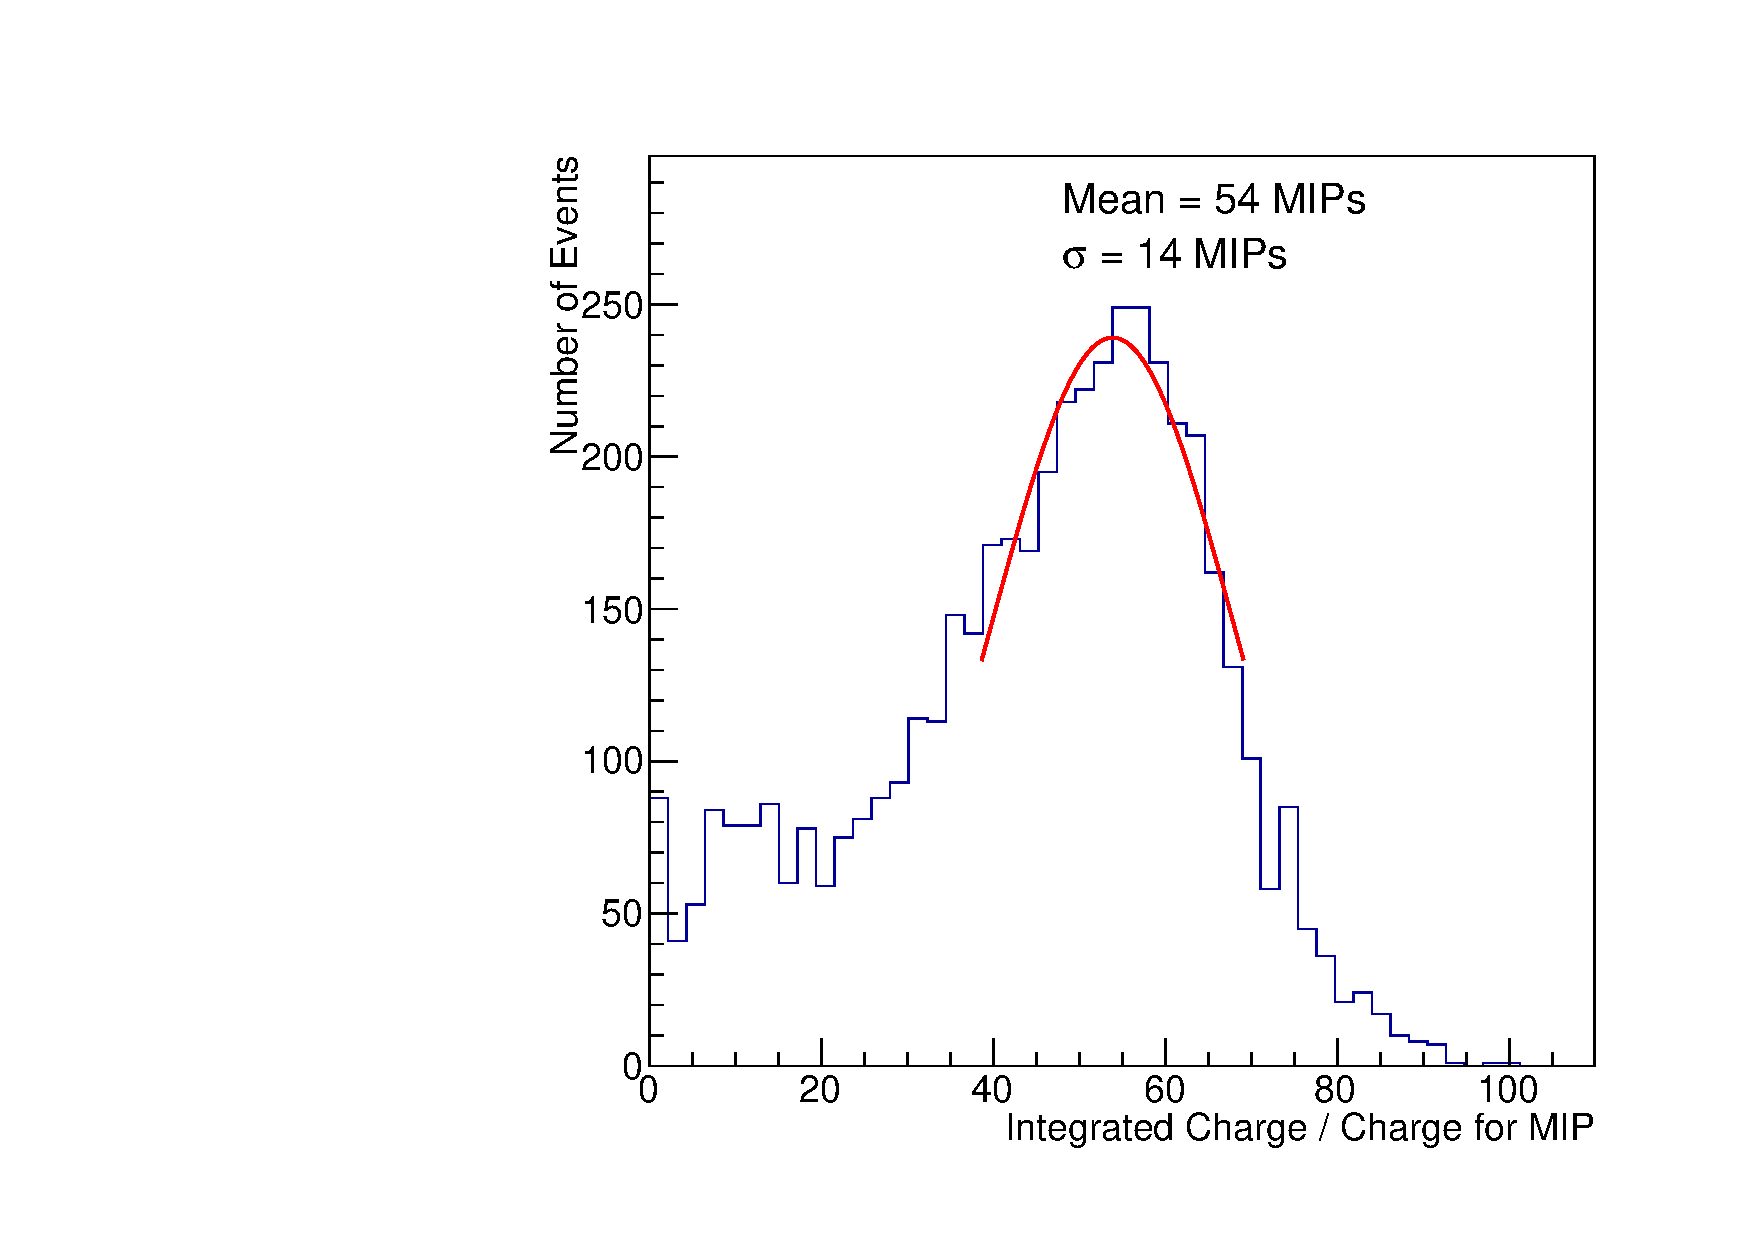
\includegraphics[width=0.49\textwidth]{plots/Electron_6X0_32GeV_chargeMIP.pdf} 
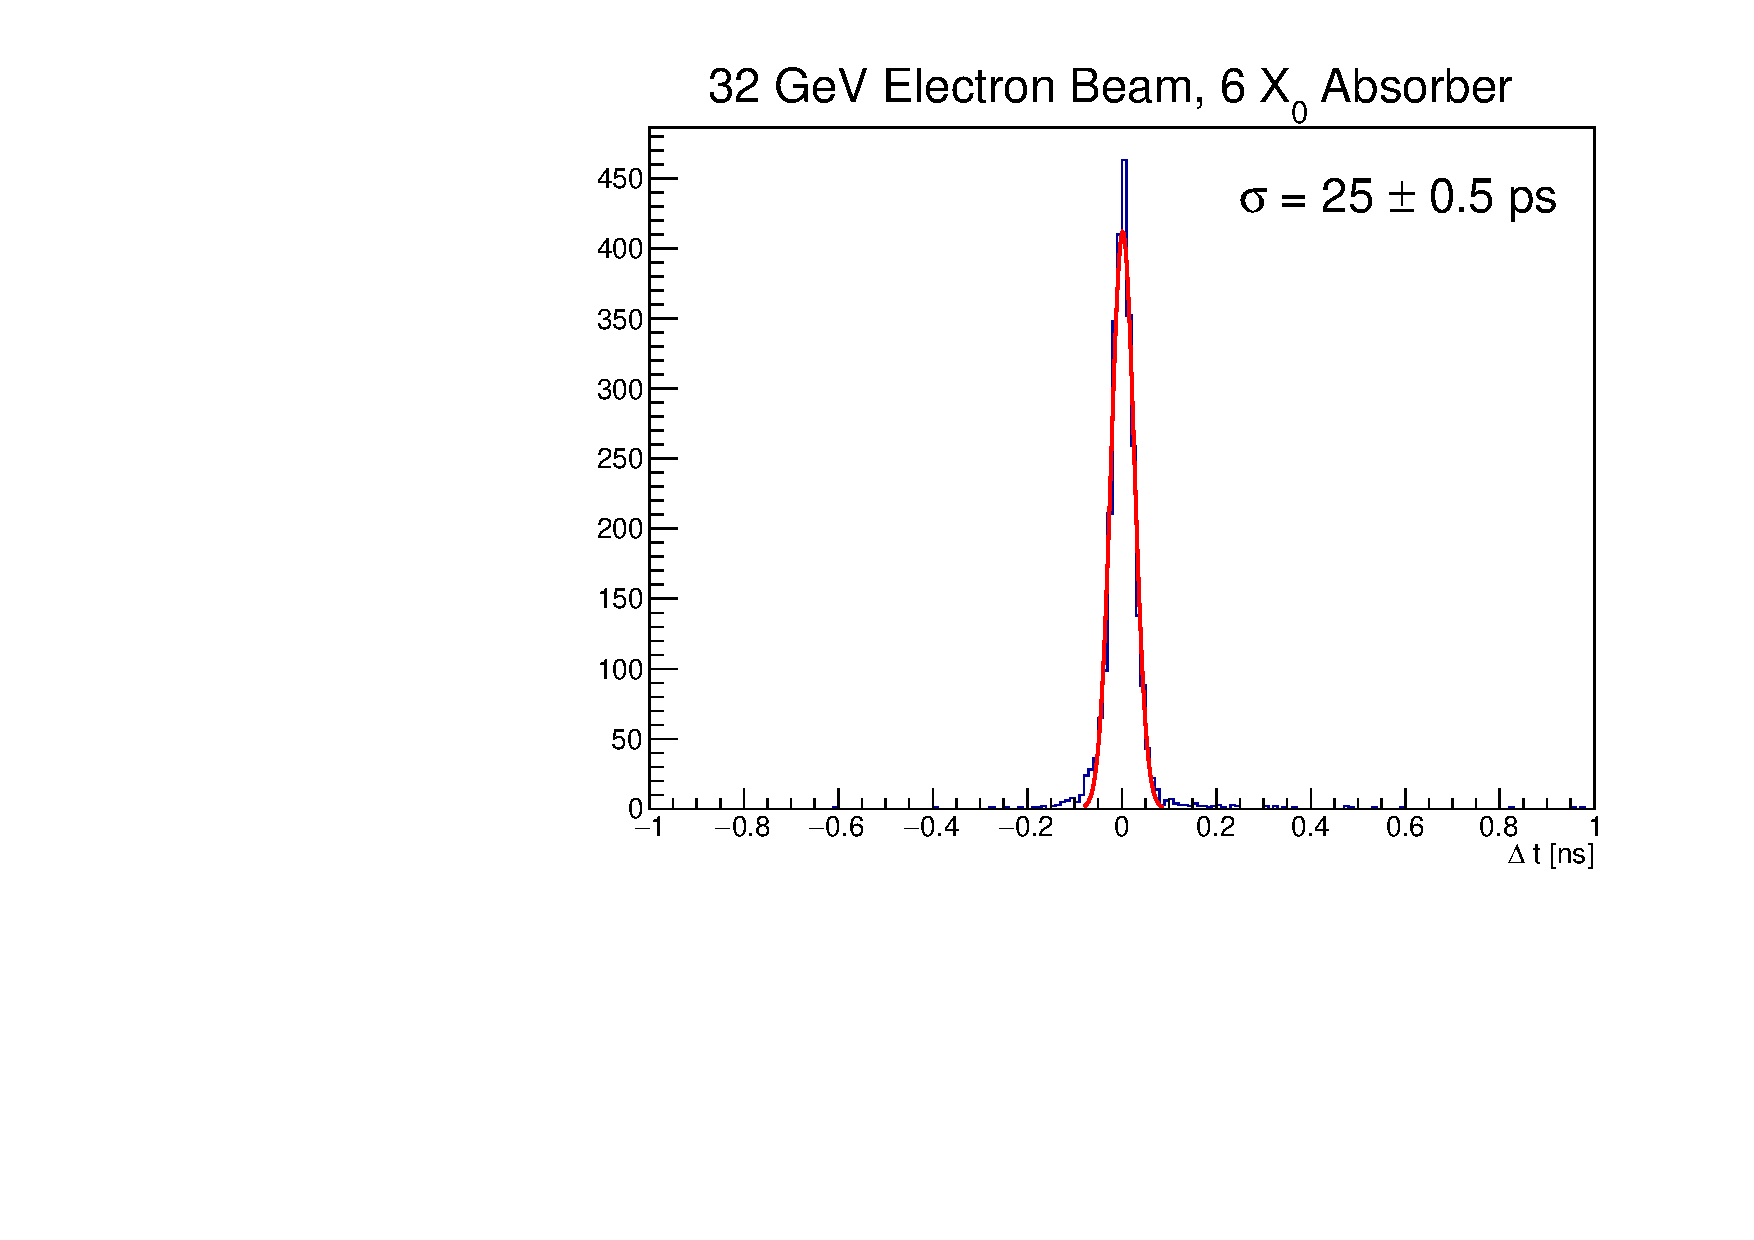
\includegraphics[width=0.50\textwidth]{plots/deltaT_32GeV_6X0.pdf} 
\caption{ An example of the distribution of integrated charge in the silicon sensor is 
shown in units of the charge measured for MIP's. A 32 GeV electron beam is used, and the
silicon sensor is placed after 6 radiation lengths of tungsten absorber.} 
\label{fig:ChargeDistributionExample}
\end{figure}

\begin{figure}[htbp] 
\centering
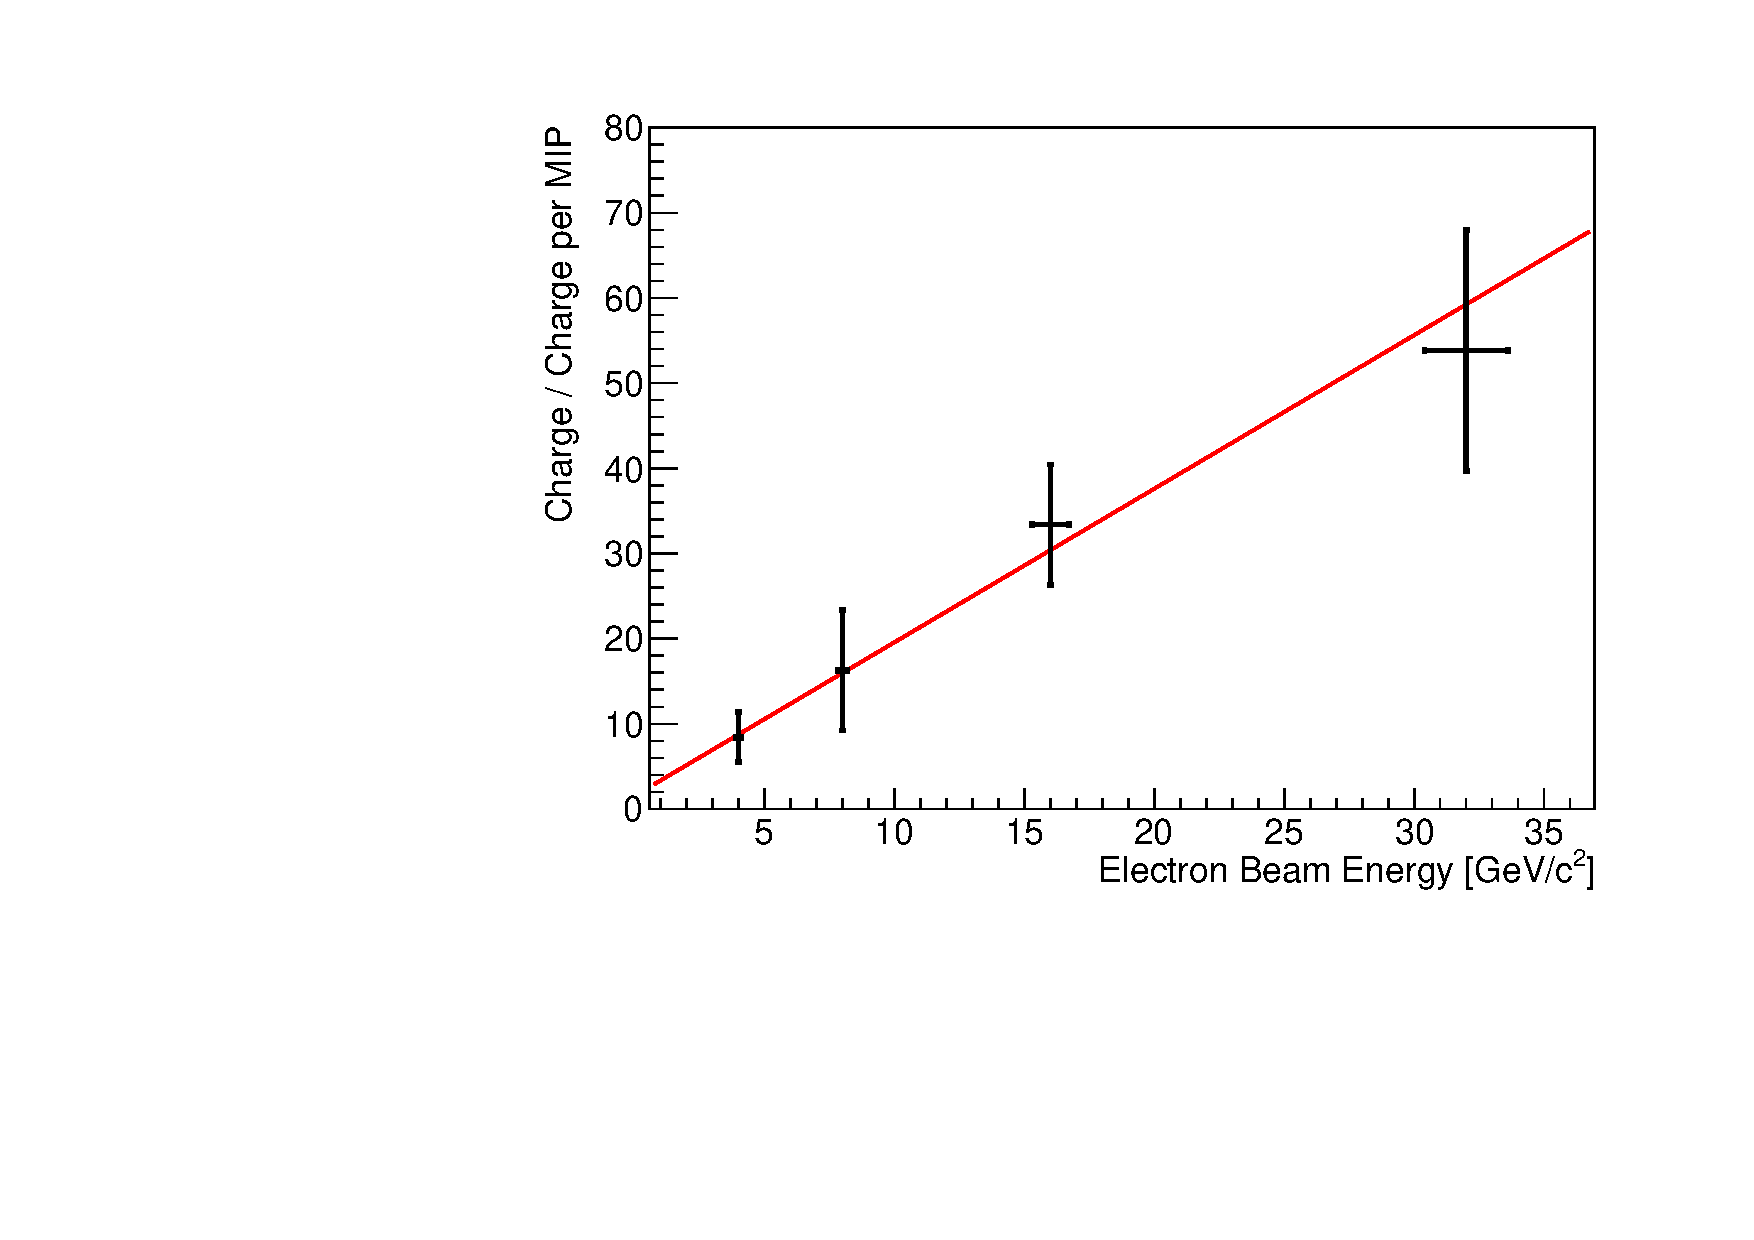
\includegraphics[width=0.49\textwidth]{plots/MIPVsEnergyAt6X0.pdf} 
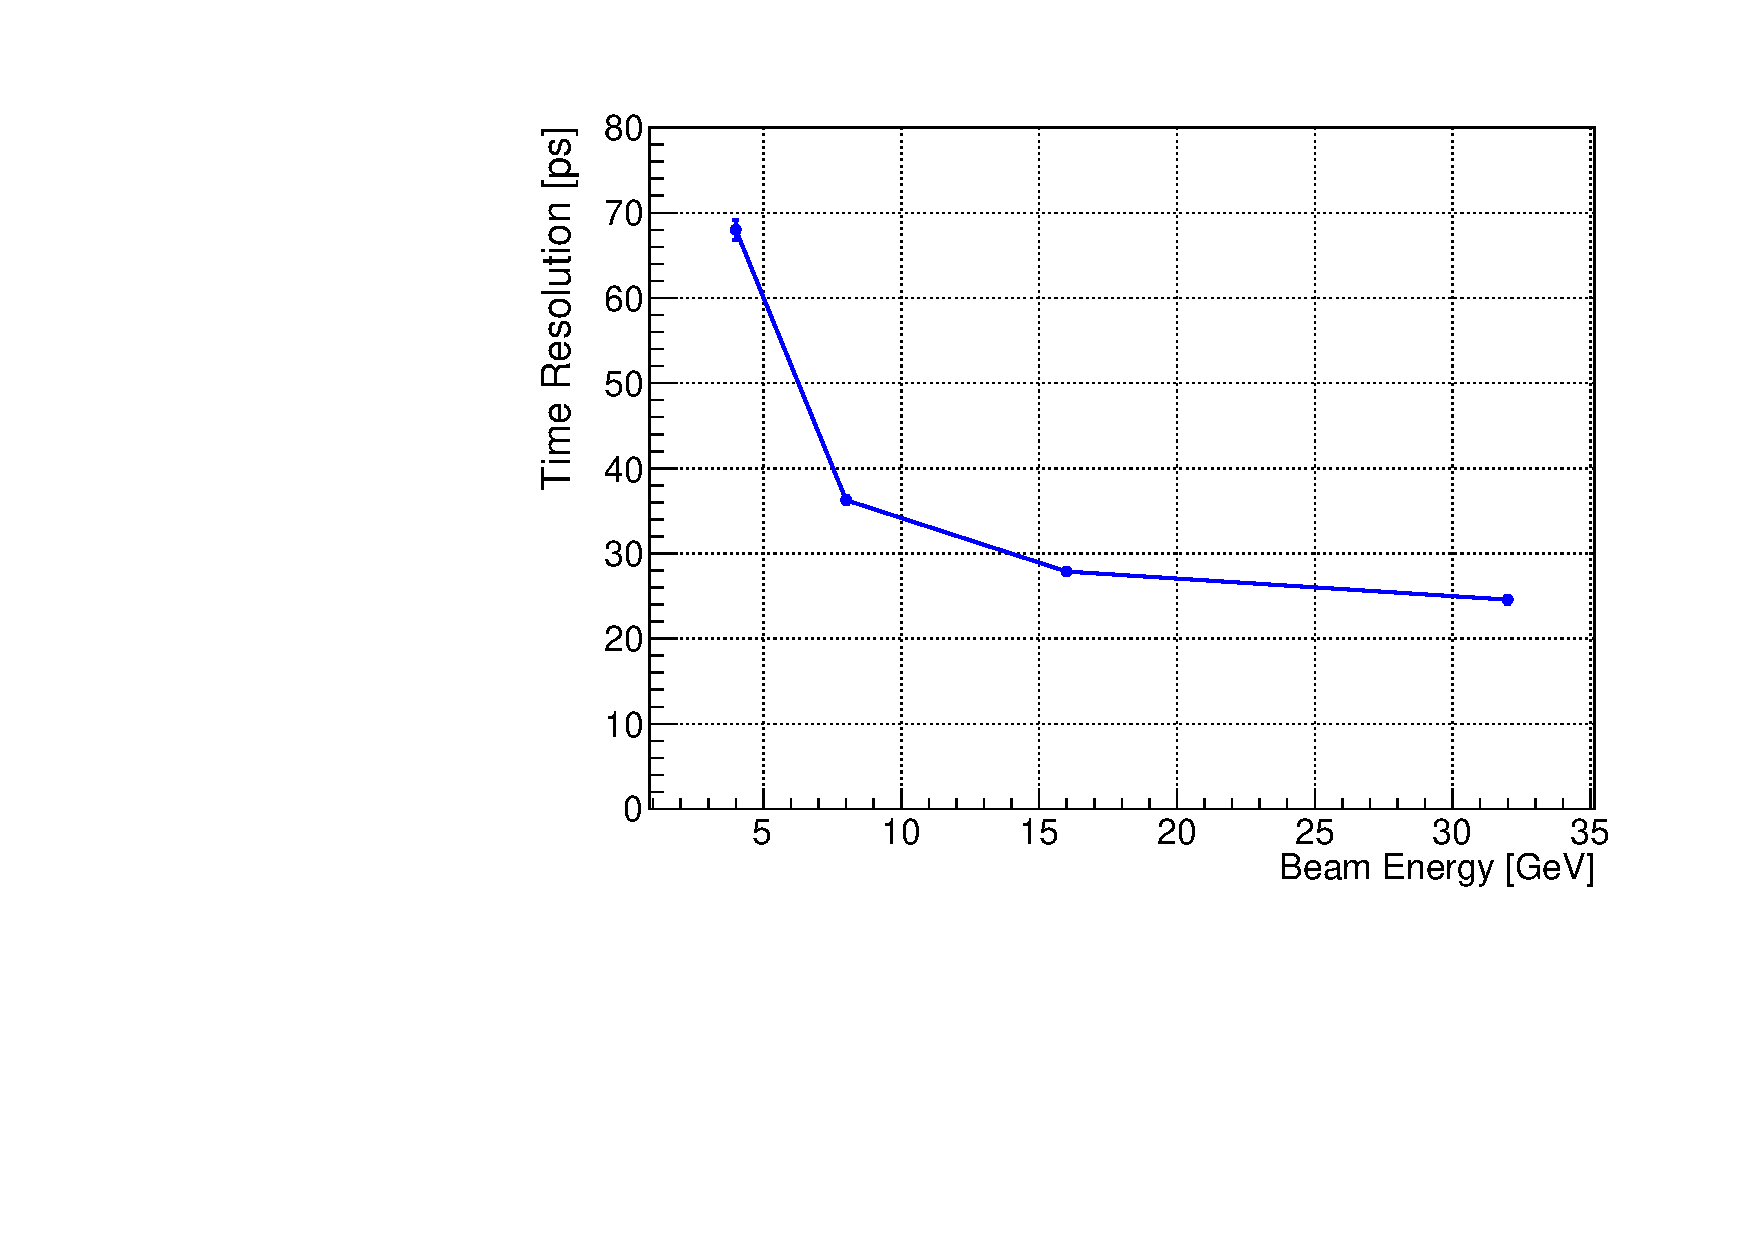
\includegraphics[width=0.50\textwidth]{plots/SigmaT_vs_BeamEnergy_lin30Stamp.pdf} 
\caption{On the left, the integrated charge in the silicon sensor expressed in units of the 
charge measured for MIP's is shown as a function of the electron beam energy. The uncertainty
bands show the RMS of the measured charge distribution. The red line is the best fit to a 
linear function. On the right, the measured time resolution between the silicon sensor and the 
Photek MCP-PMT reference is shown as a function of the electron beam energy.
} 
\label{fig:MIPVsEnergy} 
\end{figure} 

We also measure the time resolution between the silicon sensor and the Photek MCP-PMT.
An example of the time of flight distribution is shown on the right of 
Figure~\ref{fig:ChargeDistributionExample} for $32$~GeV electrons after 6 radiation
lengths of tungsten. The dependence of the measured time resolution on the beam
energy is shown on the right of Figure~\ref{fig:MIPVsEnergy}. We observe an improvement
in the time resolution as beam energy increases, and achieve a time resolution of $23$~ps
for the $32$~GeV electron beam. 

Furthermore, we study the response and time resolution of the silicon sensor
along the longitudinal direction of the shower development. We measure the
integrated charge and the time resolution as a function of the absorber thickness
and present the results in Figure~\ref{fig:MIPVsAbsorberAt8GeV}. A typical 
longitudinal shower profile is observed, consistent with previous studies performed
using a secondary emission calorimter prototype based on MCP's~\cite{MCPShowerMaxPaper},
as well as independent studies of silicon-based calorimeter prototypes~\cite{Muhuri201424}.
We also observe that the time resolution improves as the shower develops towards its 
maximum in the longitudinal direction.

\begin{figure}[htbp] 
\centering
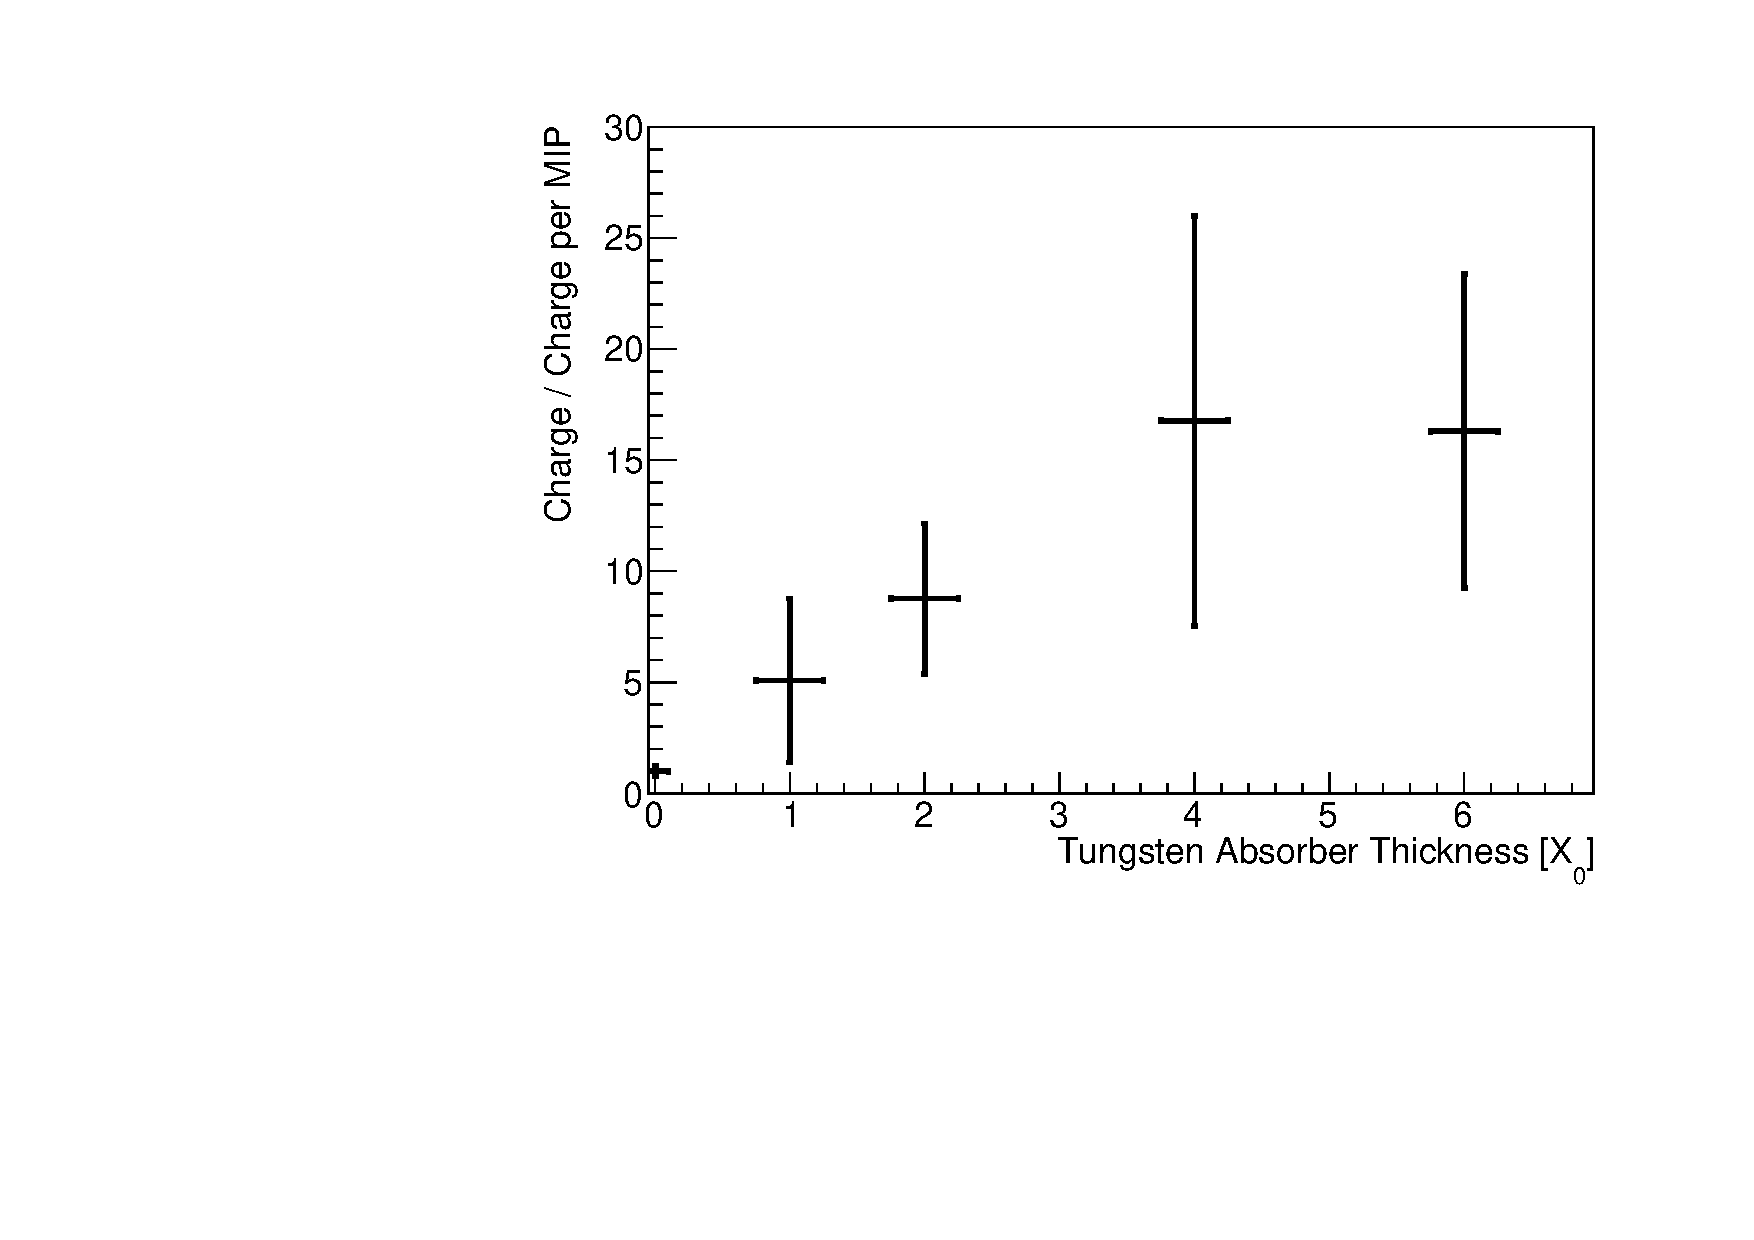
\includegraphics[width=0.49\textwidth]{plots/MIPVsAbsorberAt8GeV.pdf} 
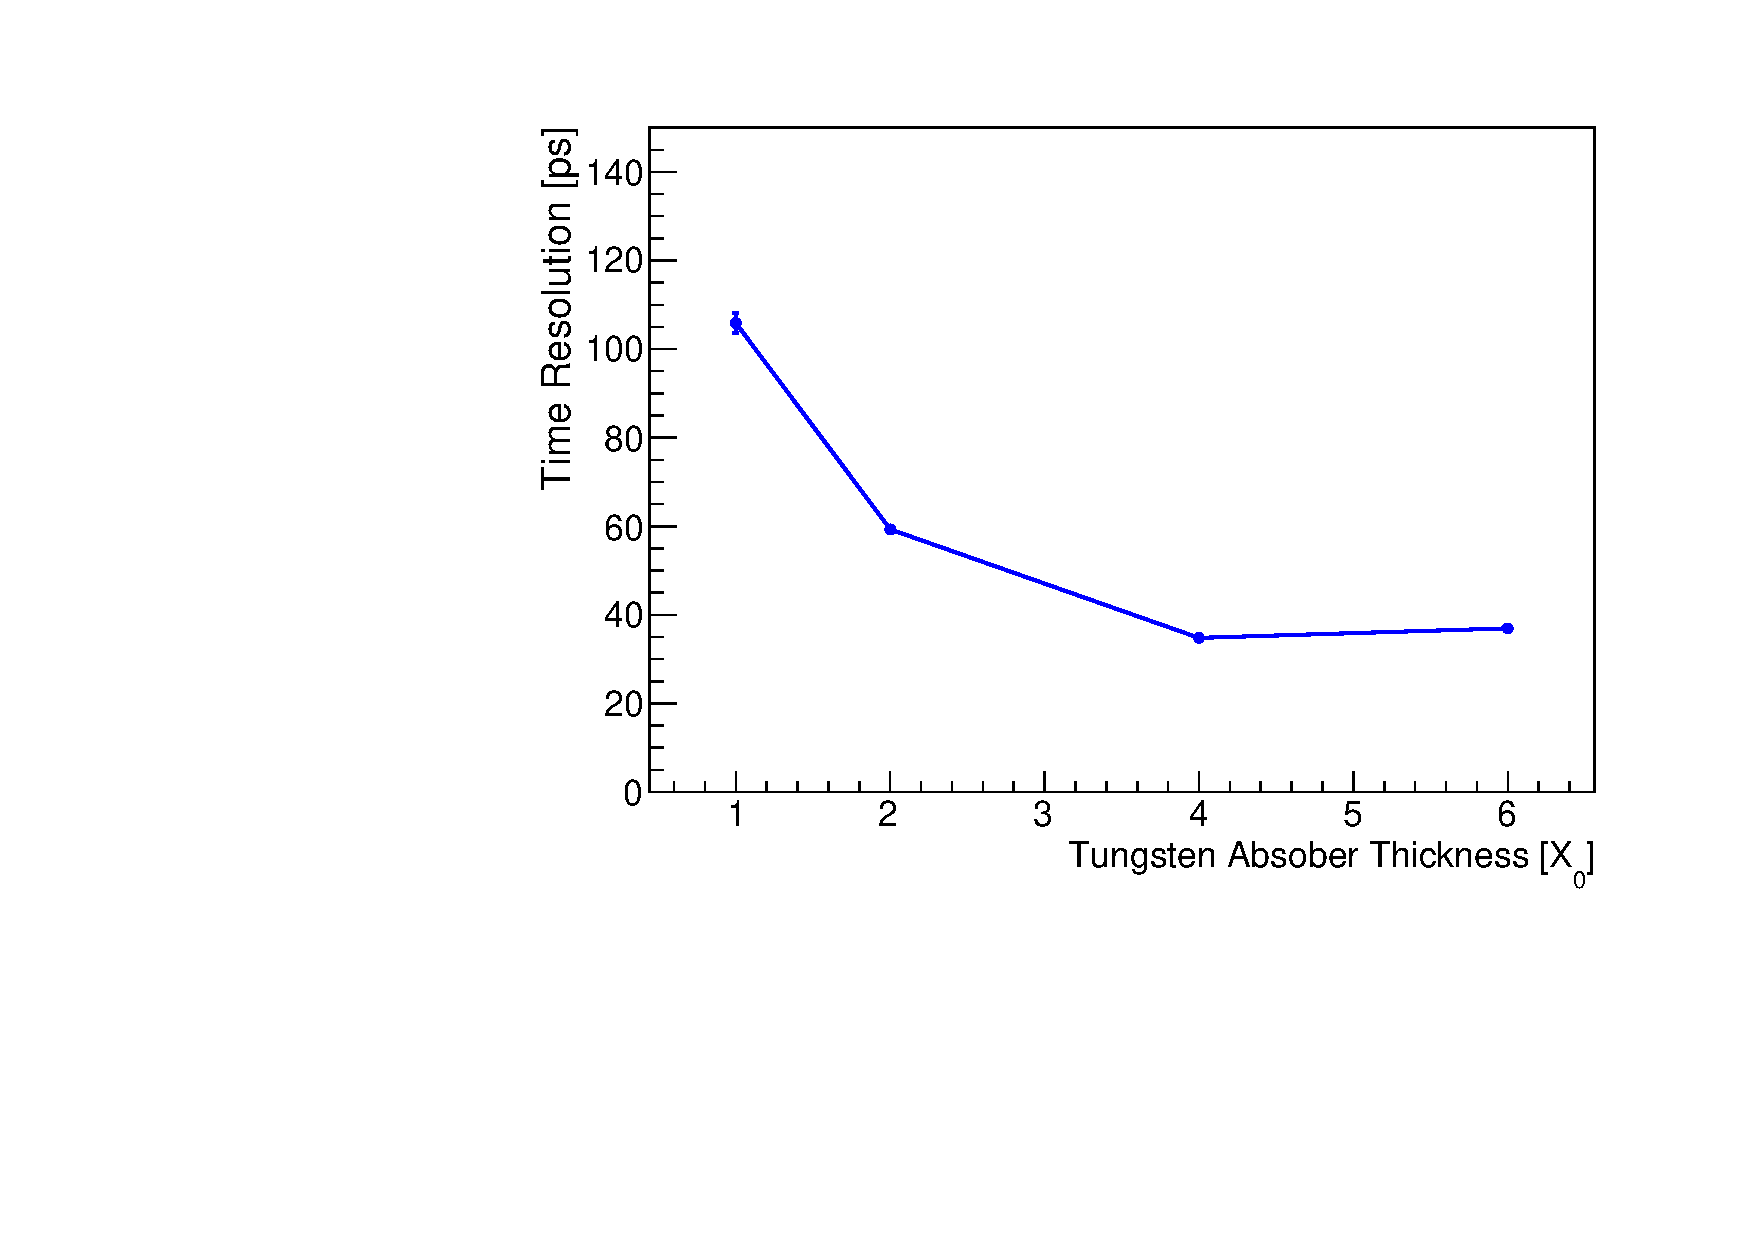
\includegraphics[width=0.5\textwidth]{plots/SigmaT_vs_X0_lin30Stamp.pdf} 
\caption{On the left, the integrated charge in the silicon sensor expressed in units of the 
charge measured for MIP's is shown as a function of the absorber (W) thickness measured in
units of radiation lengths ($X_{0}$). The uncertainty bands show the RMS of the measured charge 
distribution. On the right, the time resolution between the silicon 
sensor and the Photek MCP-PMT reference is shown as a function of the 
absorber thickness.
} 
\label{fig:MIPVsAbsorberAt8GeV} 
\end{figure} 

Finally, we studied the dependence of the time resolution as a function of the
bias voltage applied to deplete the silicon sensor. The measurements are shown
in Figure~\ref{fig:SigmaT_vs_DV_lin30Stamp} for $16$~GeV electrons after
6 radiation lengths of tungsten absorber. We find that the time resolution
improves as the bias voltage is increased, which is expected on the basis of 
increased velocity of electrons and holes in silicon at larger bias voltage. 

\begin{figure}[htbp] 
\centering
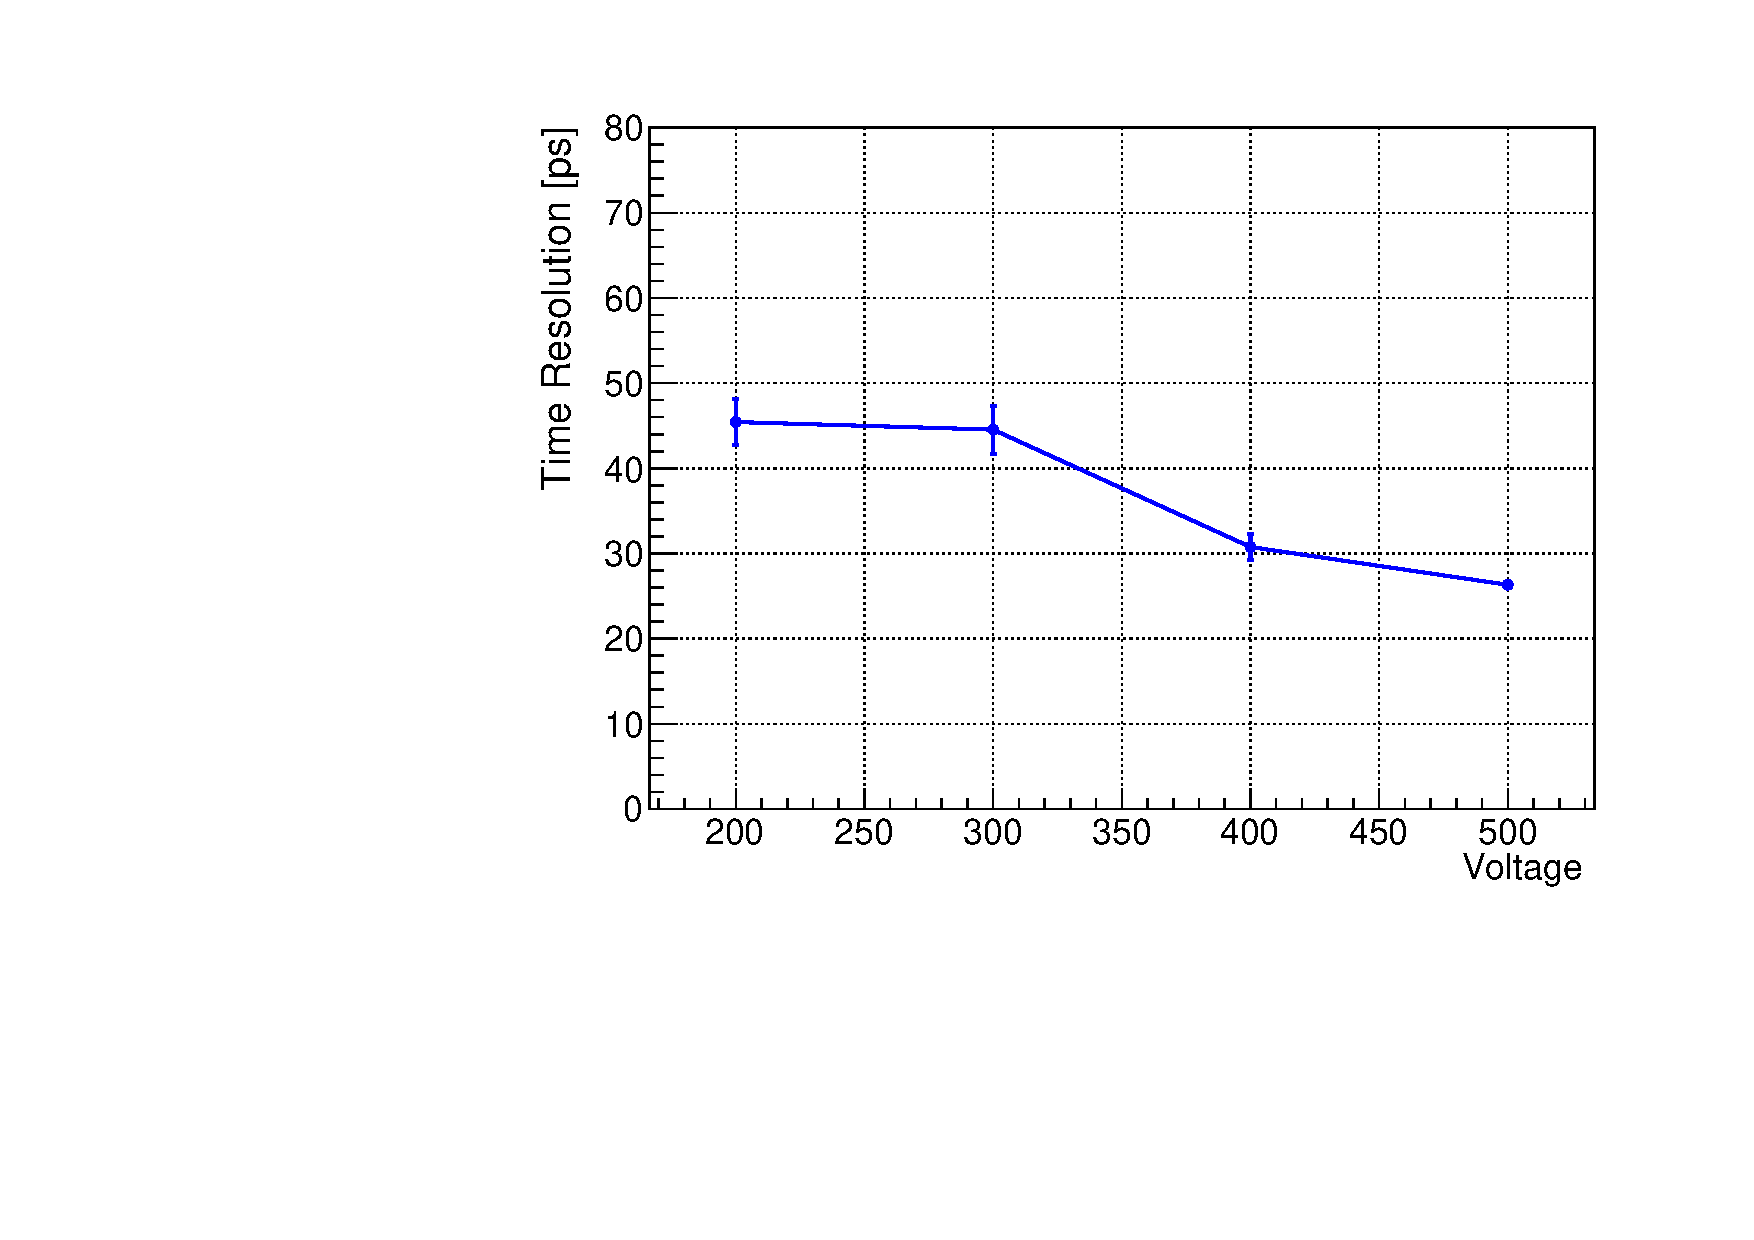
\includegraphics[width=0.8\textwidth]{plots/SigmaT_vs_DV_lin30Stamp.pdf} 
\caption{The time resolution between the silicon sensor and the Photek MCP-PMT 
reference is shown as a function of bias voltage applied on the silicon sensor. } 
\label{fig:SigmaT_vs_DV_lin30Stamp} 
\end{figure} 

\section{Discussion} 
\label{sec:discussion} 

Electric field applied to silicon results in the built-in junction voltage
(~0.6V) which is typical of silicon diodes. The high electric field in silicon
leads to total depletion which is formed from a conducting region by removal of
all free charge carriers. When charged particle pass through the totally
depleted silicon region it produces carriers collecting on corresponding
electrodes and producing output signal. Suppose the thickness of the silicon is
100 $\mu$m. The relativistic particle pass the 100~$\mu$m by 0.3~ps, so we can neglect
this time (and jitter) in the consideration. The electrons produced by the
particle collected on positive electrode and the holes on the negative. At high
fields E > 105 V/cm the mobility of carriers attain a constant drift velocity of
108~mm/s (1$\mu$m/10~ps) in the silicon [21]. The amount of electrons produced in the
100 um is ~10000 (let’s take this value instead of 8000 for simplicity). The
time needed to collect all electrons in the 100 um is ~1ns. The electrons produced closer to the positive electrode collected first. The
time needed to pass 1~$\mu$m by electron is $\sim$10~ps. The average time between the
electrons is $\sim$1~ps. If electronic can detect 100 electrons its arrival time
could be inside of the 10~ps. The time jitter could be estimated as 3~ps for
Poisson timing distribution. For example, if electronics can detects $\sim$100
electrons (with additional amplification) produced in silicon they collected
from the thickness of $\sim$10~$\mu$m. We can say that the ``rest of the silicon
thickness'' does not participate in the silicon time jitter, because these
electrons are coming ``too late''. This simple model can explain in general
obtained test beam results.The obtained data are in good consistency with calculation. The noise of the
silicon with performed schematics is pretty low. It allows to detects the 120
GeV proton and 4 GeV electron (w/o absorber) with high efficiency, which could
be estimated as $>80$\% (Figs. 6-8). The detected charge shows linear dependence
on absorber length. (Figs. 9, 10). The longitudinal shower profile performed
with the silicon is in good consistency with previous result obtained with MCP.
The integrated silicon charge in dependence on Bias voltage show saturation at
$\sim$500V for used silicon. This is $\sim 150$~V less of maximum voltage that could be
applied to the silicon. The measured and calculated time resolution for the
silicon are in good consistency (Fig. 13).


\section{Conclusion}
\label{sec:conclusion} 

We obtained time resolution for the silicon $\sim$23 ps. This could correspond to
$\sim$137 particle registered in the shower. The 120~GeV proton amplitude corresponds
to $\sim$20 mV according to measurements and estimation. We see significant amplitude
increase when absorber used. This open an opportunity to use the silicon as
active layer in calorimeter, for example in CMS HGC upgrade [22]. We can
consider the results of this work as good opportunity to use silicon for timing
measurements in future calorimeter. We plan to perform optimization of the
possible silicon version, e.g. transverse size and configuration for multipixel
readout, etc. This will be aim of our next work.


\section{Acknowledgements} We thank FTBF personnel for very good beam condition during our test run. We also appreciate technical support of Fermilab SiDet department for production of high quality silicon samples. We appreciate Helmuth Spieler monography as a good source of silicon information [23].

\bibliography{SiliconCalorimeter}{}
\bibliographystyle{ieeetr} 

\end{document}





















